\documentclass{article}
\usepackage[utf8]{inputenc}
\usepackage{graphicx}
\graphicspath{ {images/} }
\usepackage{hyperref}
\usepackage{xcolor}

\title{How I organize research code}
\author{Robby Parker}
\date{September 2022}

\begin{document}

\maketitle

\section{Motivation}
Computational research involves writing many different pieces of code.
Often, when writing a new piece of code, I find myself wondering where
to put it. And then wondering when it is ``good enough'' to be promoted.
This document presents and describes the different repositories that I
use to manage code for different projects, at different levels of
maturity.

This is just a system that I have developed to categorize the code that
I write. I don't necessarily intend for anybody to copy the repositories
I use, but if any of this document helps anybody think about how to
structure their own research software, it has served its purpose.

Admittedly, some of this is specific to Python, the programming language
I have used for my PhD (e.g. ``update imports'', ``structured as a
Python package''). However, I think the general concepts should apply to
research software in any language.

\section{Different repositories}

\hspace{-1.5cm}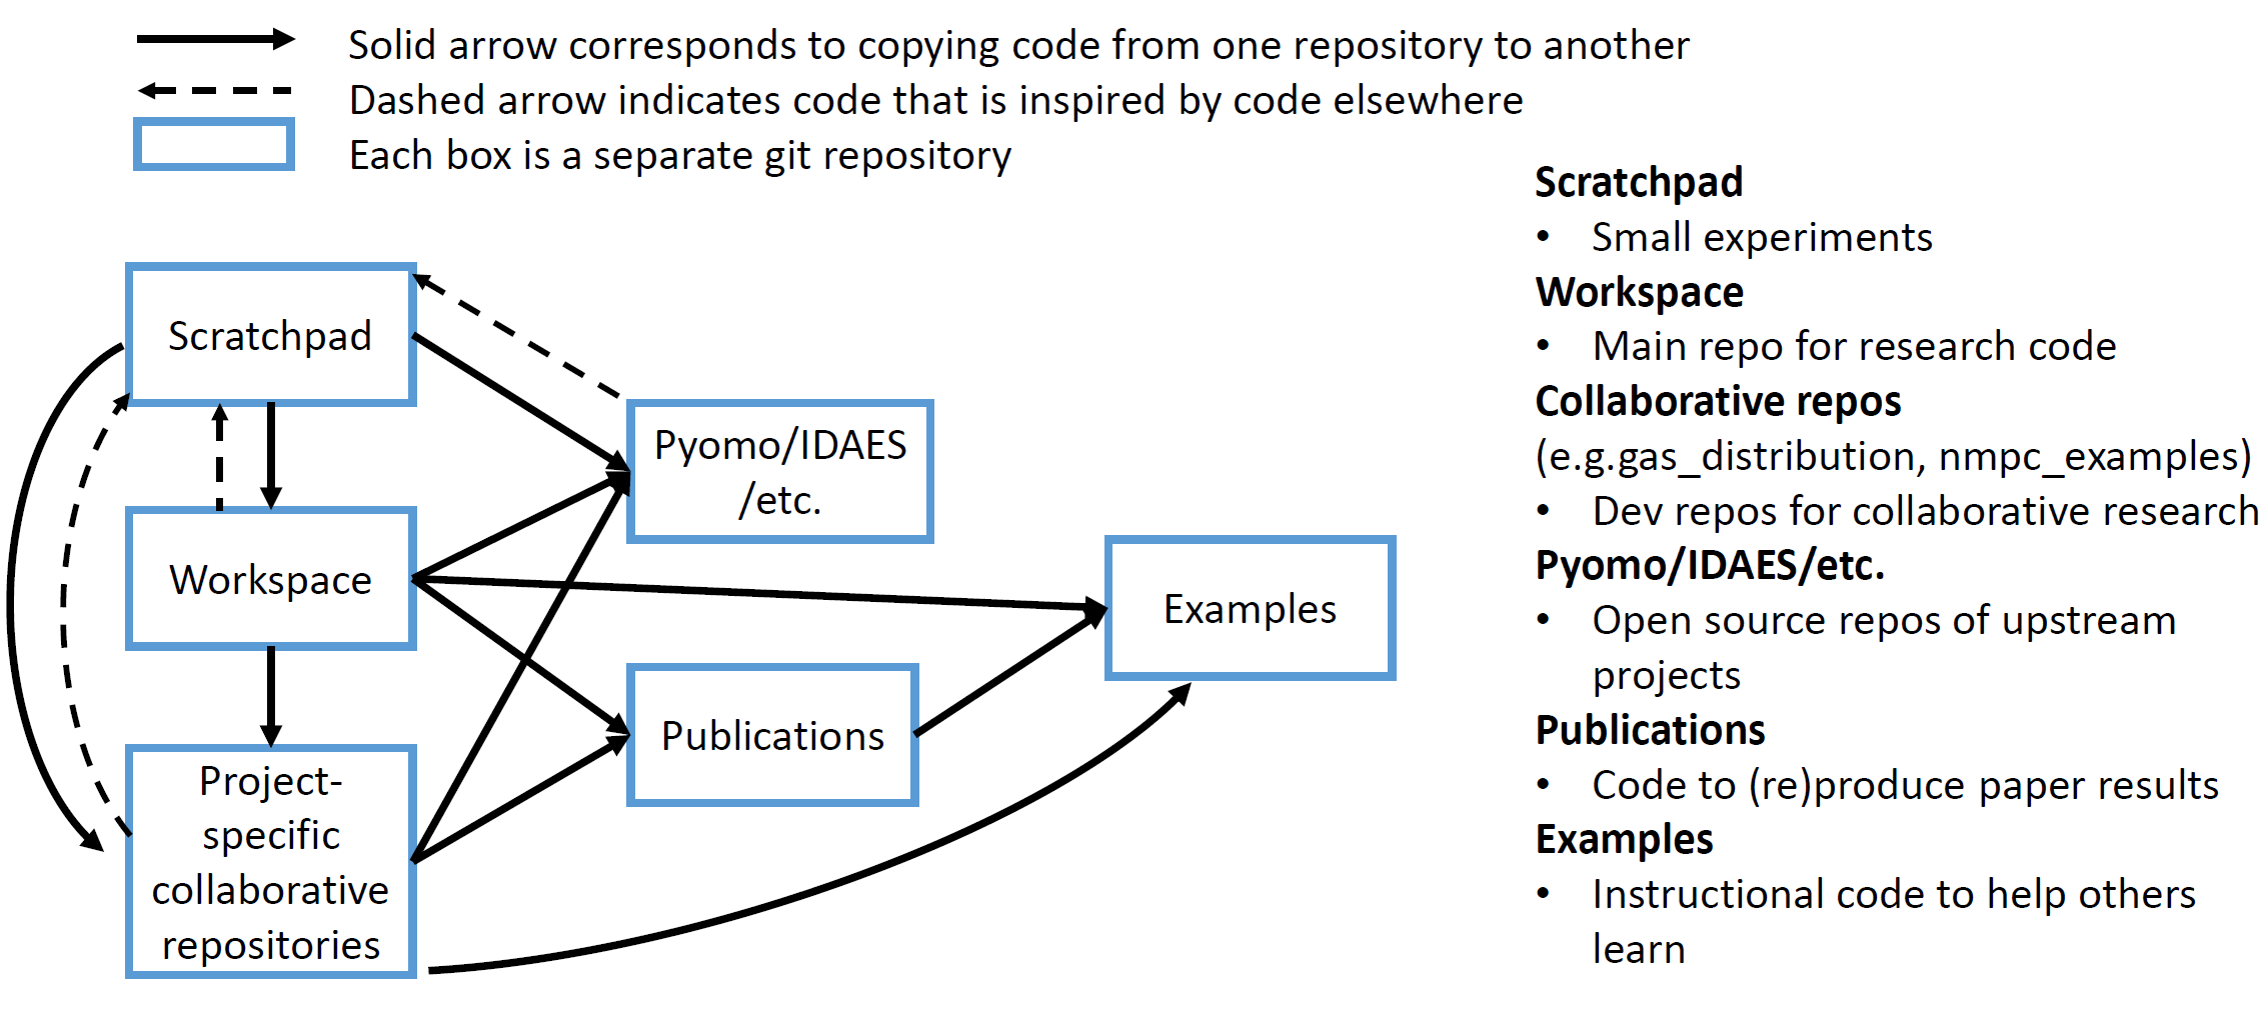
\includegraphics[width=15cm]{repo_diagram}

Most code starts out in workspace, either as a utility method/class,
implementation an algorithm, or model/case study.
It then gets promoted through one of several pathways:
\begin{itemize}
  \item Copied to the repo of an upstream open-source project (e.g. Pyomo,
    IDAES) for PR, review, and eventual merge
  \item Copied into its own repository for collaborative development
  \item Copied into a dedicated repository for publications when it is
    being used for paper results
  \item Copied into a dedicated repository for examples (of some tool
    or algorithm)
\end{itemize}

\noindent Criteria with which to compare repositories:
\begin{itemize}
  \item Private or public?
  \item Do I commonly (ever) make new branches?
  \item Testing requirement for code in the repo
  \item Documentation requirement for code in the repo
  \item Structured as a package? (I.e. can I import from it?)
\end{itemize}

\section{Scratchpad}
\begin{itemize}
  \item Private repo
  \item Doesn't use branches
  \item Testing requirement: None
  \item Documentation requirement: None
\end{itemize}
A repository for running small examples, testing new features, and
debugging. I often use this to write a small script to test a new
Pyomo feature or test something while reviewing a PR.

\begin{center}
  \newpage
  Sample scratchpad directory structure\\
  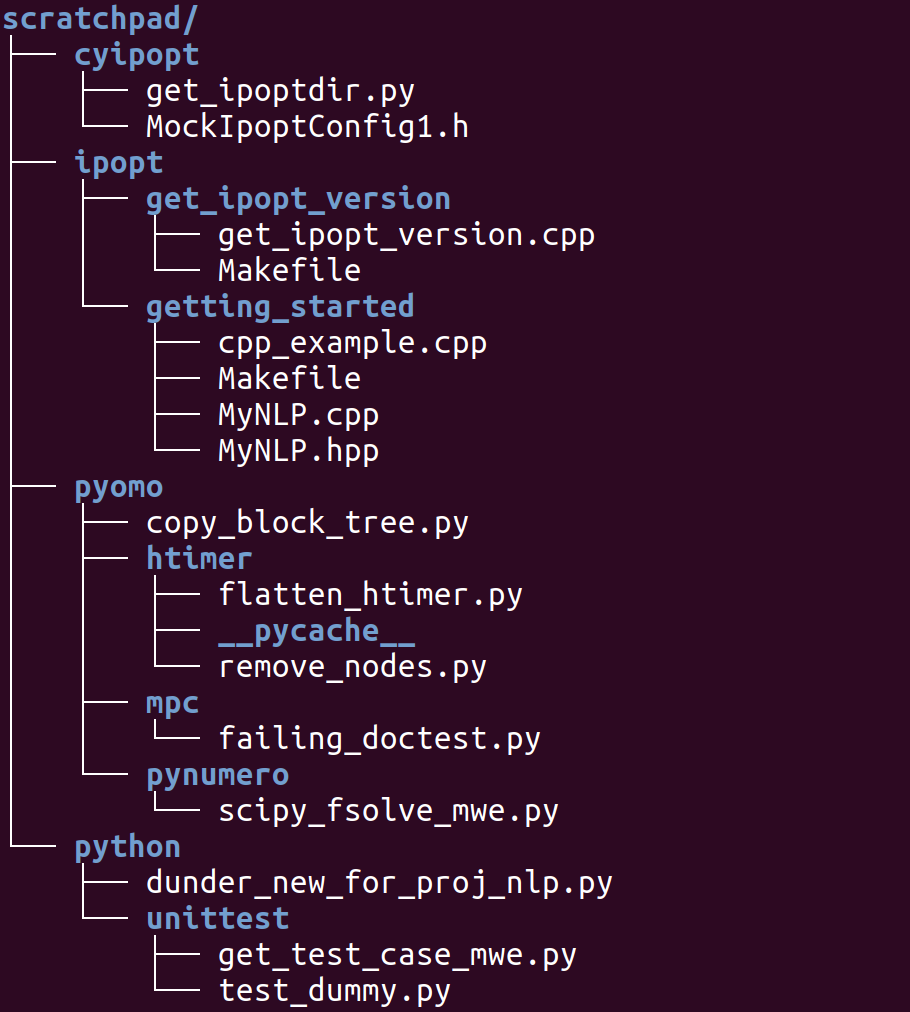
\includegraphics[width=8cm]{scratchpad_tree.png}
\end{center}

Several of the files in my scratchpad repository are just minimal
working examples of bugs/issues/features -- this is a large portion
of what I use this repo for.

\section{Workspace}
\begin{itemize}
  \item Private repo
  \item Doesn't use branches
  \item Testing requirement: {\color{purple}\bf medium}
  \item Documentation requirement: {\color{blue}\bf low}
  \item Structured as a Python package
\end{itemize}
My main repository for research development. I have different
directories for each model I work on and different repositories for
each tool/algorithm I'm working on.
The repo is structured as a Python package as I am constantly
importing code from different locations within the repo,
including in tests.
I find tests to be a pretty critical part of this repository. While
I don't necessarily write unit tests to cover every line of code,
when I come back to a project for the first time in a while, it is
pretty useful to be able to run a single command to make sure
my code still works.
\begin{center}
  Sample (first two levels of) workspace directory structure\\
  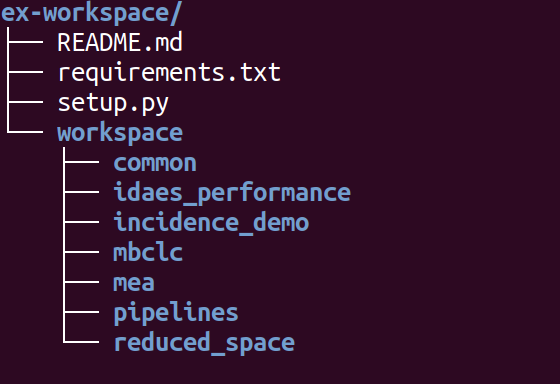
\includegraphics[width=6cm]{workspace_tree.png}
  \\
  Directory structure of the \texttt{incidence\_demo/} subdirectory
  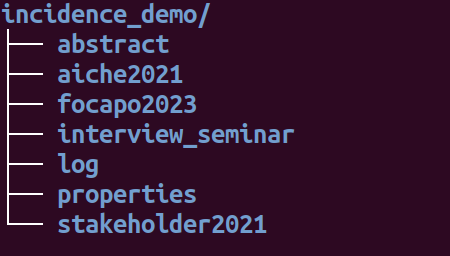
\includegraphics[width=7cm]{incidence_demo_tree.png}
\end{center}

You can see I make a new directory every time I make a presentation or
paper about or including the incidence graph work I've done.

\section{Single-project collaborative repositories}
For example,
\href{https://github.com/Robbybp/gas_distribution}{\texttt{gas\_distribution}}
or
\href{https://github.com/robbybp/nmpc_examples}{\texttt{nmpc\_examples}}.
\begin{itemize}
  \item Only private if sensitive data is involved
  \item Use branches
  \item Testing requirement: {\color{purple}\bf medium}
  \item Documentation requirement: {\color{blue}\bf low}
  \item Structured as Python packages
\end{itemize}
When actively collaborating with others on research code, we create
a dedicated repository for the project, rather than just sharing a
``workspace'' directory, which contains way more code than somebody else
wants to look through.
These repositories can start out with code copied from workspace
(if somebody starts collaborating after I have started working on something)
or as empty repositories (if I start a new project knowing it will be
collaborative).

\begin{center}
  First two levels of the directory structure of \texttt{gas\_distribution}
  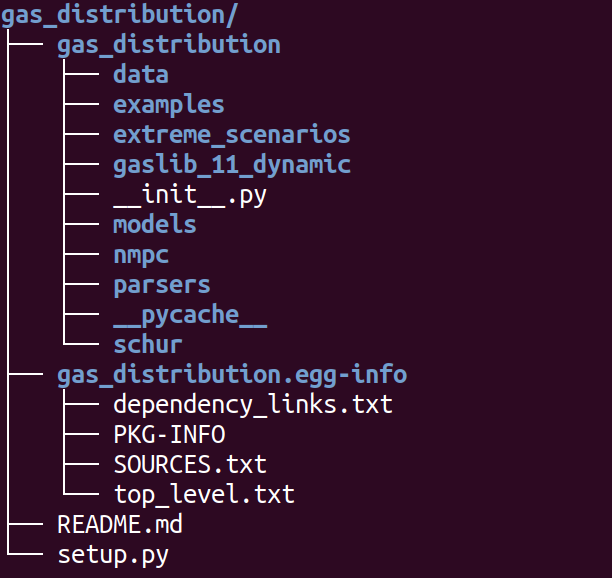
\includegraphics[width=7cm]{gas_distribution_tree.png}
\end{center}

This is basically just one of the problem-specific subdirectories of
workspace, now with branching and PRs, etc.

\section{Upstream open-source repositories}
For example, Pyomo or IDAES.
\begin{itemize}
  \item Public
  \item Use branches
  \item Testing requirement: {\color{red}\bf high}
  \item Documentation requirement: {\color{red}\bf high}
  \item Are Python packages
\end{itemize}

These are pretty self-explanatory. When I have code that I think
is useful, clear, maintainable, and would make a valuable
contribution to an upstream project, I copy the code into a branch
of one of these repositories, write some tests, and open a PR.
Or if I'm working on a feature or fix for an upstream project,
I'll start out my development in a branch of one of these
repositories.

\section{Publications}
For example, \href{https://github.com/idaes/publications}{IDAES/publications}.
\begin{itemize}
  \item Public
  \item Use branches
  \item Testing requirement: {\color{purple}\bf medium}
  \item Documentation requirement: {\color{purple}\bf medium}
  \item Code for each paper is structured as a package
  \item No unreleased dependencies!
\end{itemize}

When a tool, algorithm, or case study gets to the point where it is
ready for a paper, I copy the code into a separate repository for
publications in a directory named for something to do with the paper.
The purpose of this is to help a reader or reviewer reproduce the
results (and if they are ambitious, see what's actually going on
in the code).
It needs to be documented well enough that somebody knows what to run
to produce results (e.g. plots), and preferably has some tests a
user can run to make sure they have the right dependencies
(and versions thereof) installed.

I try to be pretty strict about not requiring any unreleased software
to run the code in this repository (e.g. saying ``go checkout my branch
of Pyomo'').

Since this code is not something I want to maintain after a paper is
published, I freeze the environment I used to generate the results
(so a user knows the exact version of every dependency)
and worry about correctness for that environment only.

\begin{center}
  Sample directory structure for a publications repository.\\
  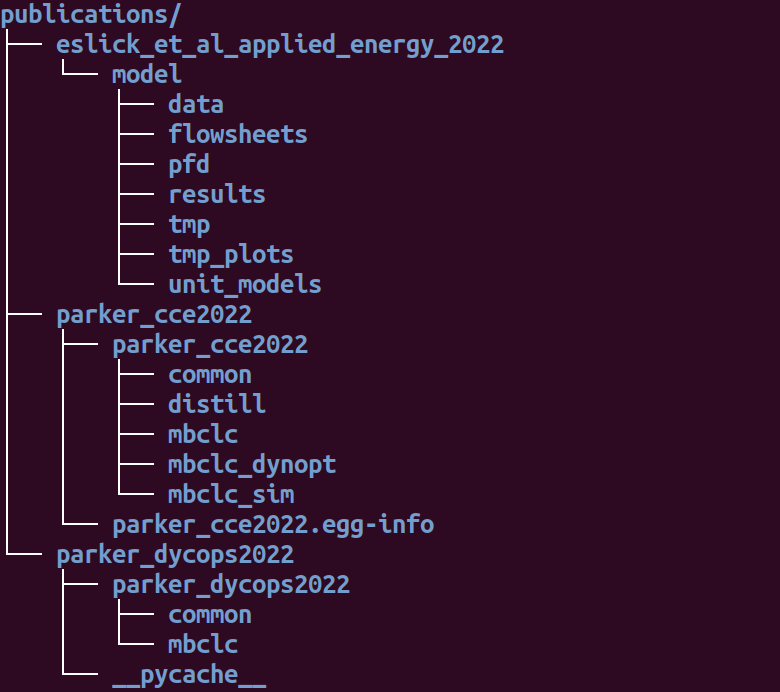
\includegraphics[width=10cm]{publications_tree}
\end{center}

\section{Examples}
For example, \href{https://github.com/IDAES/examples-pse}{IDAES/examples-pse}
or \href{https://github.com/Robbybp/incidence_examples}{\texttt{incidence\_examples}}.
\begin{itemize}
  \item Public
  \item Uses branches
  \item Testing requirement: {\color{red}\bf high}
  \item Documentation requirement: {\color{red}\bf high}
\end{itemize}

When some code that does something useful is concise and explainable
enough to be read, understood, and learned from, it might make a good
example. To me, examples should have the strictest requirements requirements
of any of the pieces of code I've covered, as they need to be not only
well-tested and well-documented, but the code itself needs to be
understandable enough to make for good learning/explanation material.

I don't have a lot of experience writing examples --
\href{https://github.com/Robbybp/incidence_examples}{\texttt{incidence\_examples}}
is my only real attempt. Some projects include examples in the main project
repository, while some distribute them as a separate repo.
I don't have a strong opinion about this, as long as they can be tested
for every PR in the main repository.
Examples also seem to come in either scripts or (Jupyter) notebooks.
I prefer scripts, but admit that notebooks have benefits for demonstrations.

\begin{center}
  Sample directory structure for an examples repository.\\
  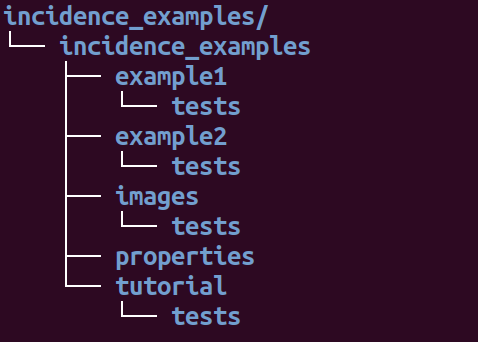
\includegraphics[width=6cm]{incidence_examples_tree_small}
\end{center}

\section{General tips}
Some unsolicited advice.

\subsection{Don't maintain the same code multiple places}
Once you've ``promoted'' code by copying to another repository
(e.g. repo for collaborative work, or upstream open-source repo),
don't maintain it in the original location.
Ideally, update imports to use the code in the new location,
run the tests to make sure it works, and delete the old code.

\subsection{Update imports (and function names) with
\texttt{find} and \texttt{sed}}
Using \texttt{find} and \texttt{sed} to do simple replacement
for all files in a directory tree should be be second-nature.

Common commands:
\begin{itemize}
  \item \texttt{grep -r old\_name}\\
    To see where the old name is being used.
  \item \texttt{\small
      find . -name '*$\backslash$.py' -exec sed s/old\_name/new\_name/g \{\} $\backslash$; | grep new\_name
    }\\
    To replace the old name with the new name, then see where the new name appears.
    Make sure this is exactly where you expect.
  \item \texttt{find . -name '*$\backslash$.py' -exec sed -i s/old\_name/new\_name/g \{\} $\backslash$;
    }\\
    To actually do the replacement in-place (modify the files).
\end{itemize}

\subsection{Write tests for everything}
Having good tests for research code is amazingly useful.
When you make a change, or come back to some code after a while
and forget some of the details, being able to run tests and be reasonably
convinced it still works is a life-saver.

Good tests run quickly ($< 10$s, ideally) and exercise all the code you
are interested in. For example, when writing a model predictive control case
study, I usually write a test that constructs a small (short time horizon)
instance of my model and runs one iteration of MPC (perhaps with a simplified
setpoint/disturbance). I then test that the control variables computed are
what I expect (within tolerance).

I don't necessarily recommend unit tests for every single piece of research
code you ever write, but fast tests that tell you whether your software
works are amazing to have.

\subsection{Use your editor to its full capacity}
And the command line, for that matter.\\

E.g. find and replace, copy/cut/paste, delete/replace a word or line,
jump to the beginning or end of a word/line/paragraph, scroll through a file,
edit multiple lines at once, repeat at command or keystroke, call another
program, etc. without your hands leaving the keyboard.

\subsection{Keep a ``living document'' for each project}
I keep a \texttt{log.tex} file for every project I work on to record
my thoughts and plans, sectioned by date in reverse-chronological order.
Essentially just lab notebooks.
90\% of the value proposition of these files is just to answer the question
``What was I working on last time I touched this project?''
They're also useful places to put intermediate results that I may want to
reference at some point.

\end{document}
